\documentclass[11pt,final]{article}

\usepackage[a4paper,margin=1in]{geometry}
\usepackage{amsmath,amssymb}
\usepackage[final]{graphicx}
\usepackage{hyperref}
\usepackage{float}
\usepackage{microtype}

\title{Critical Horizon Transitions in Quadratic $f(R)$ Gravity:\\
A Topological Integrity Perspective}

\author{Kai Stefan Dietrich\\
Independent Research}

\date{May 2026}

\begin{document}

\maketitle

\begin{abstract}
We investigate a structurally controlled mechanism for horizon formation in quadratic $f(R)$ gravity with regularized mass profiles. Within a static, spherically symmetric framework, we show that the existence of horizons is governed by a critical transition controlled by a dimensionless parameter $\beta$.

The transition is traced to the algebraic structure of the horizon equation, whose roots exhibit a saddle-node bifurcation at a critical value $\beta_c$. At this point, the outer horizon branch terminates, leading to a non-analytic change in the causal structure.

Near the critical regime, the metric function develops an extended near-zero region, enhancing the tortoise coordinate and causing the echo delay time to diverge as $\beta \to \beta_c$. This corresponds to the emergence of an effectively infinite optical cavity.

The framework interpolates between classical black hole geometries and regular horizonless compact objects. Observable consequences include deviations in black hole shadow radii, shifts in quasi-normal mode spectra, and characteristic gravitational-wave echo signatures.
\end{abstract}

\section{Introduction}

General Relativity remains the foundation of modern gravitational physics \cite{einstein1915,wald1984}. Extensions such as $f(R)$ gravity introduce higher-curvature corrections and additional degrees of freedom \cite{sotiriou2010,defelice2010}.

Regular black hole geometries have been studied as alternatives to singular solutions \cite{bardeen1968,hayward2006}. Quasi-normal modes and gravitational-wave echoes provide observational channels for probing compact-object structure \cite{kokkotas1999,berti2009,cardoso2017echo,cardoso2017status}.

In this work, we study a quadratic $f(R)$ compact-object model in which horizon formation is controlled by a critical parameter. The resulting transition separates horizon-bearing configurations from horizonless regular geometries.

\section{Quadratic $f(R)$ Framework}

We consider the action
\begin{equation}
S=\int d^4x\sqrt{-g}
\left[
\frac{1}{16\pi}
\left(R-2\Lambda+\alpha R^2\right)
\right]
+S_{\mathrm{matter}} .
\end{equation}

Equivalently,
\begin{equation}
f(R)=R-2\Lambda+\mu R^2 ,
\qquad
\mu=16\pi\alpha .
\end{equation}

The additional scalar degree of freedom is
\begin{equation}
\phi=f'(R)=1+2\mu R ,
\end{equation}
with effective mass
\begin{equation}
m_\phi^2=\frac{1}{3f''(R)}=\frac{1}{6\mu}.
\end{equation}

For $\mu>0$, this scalar mode is non-tachyonic.

\section{Effective Geometry}

We consider a static, spherically symmetric metric
\begin{equation}
ds^2=-F(r)dt^2+\frac{dr^2}{F(r)}+r^2d\Omega^2 .
\end{equation}

The effective mass profile is chosen as
\begin{equation}
m(r)=\frac{Mr^3}{r^3+r_c^3},
\end{equation}
so that
\begin{equation}
F(r)=1-\frac{2m(r)}{r}.
\end{equation}

This profile interpolates between a regular core at small radii and Schwarzschild behavior at large radii.

\section{Critical Horizon Structure}

Horizons satisfy
\begin{equation}
F(r_H)=0 .
\end{equation}

Substituting the mass profile gives
\begin{equation}
r_H^3-2Mr_H^2+r_c^3=0 .
\end{equation}

Introducing
\begin{equation}
x=\frac{r_H}{2M},
\qquad
\beta=\frac{r_c}{2M},
\end{equation}
one obtains
\begin{equation}
x^3-x^2+\beta^3=0 .
\end{equation}

The critical value is
\begin{equation}
\beta_c=\left(\frac{4}{27}\right)^{1/3}.
\end{equation}

At $\beta=\beta_c$, two real roots merge. This corresponds to a saddle-node bifurcation and marks the transition between horizon-bearing and horizonless configurations.

\begin{figure}[H]
\centering
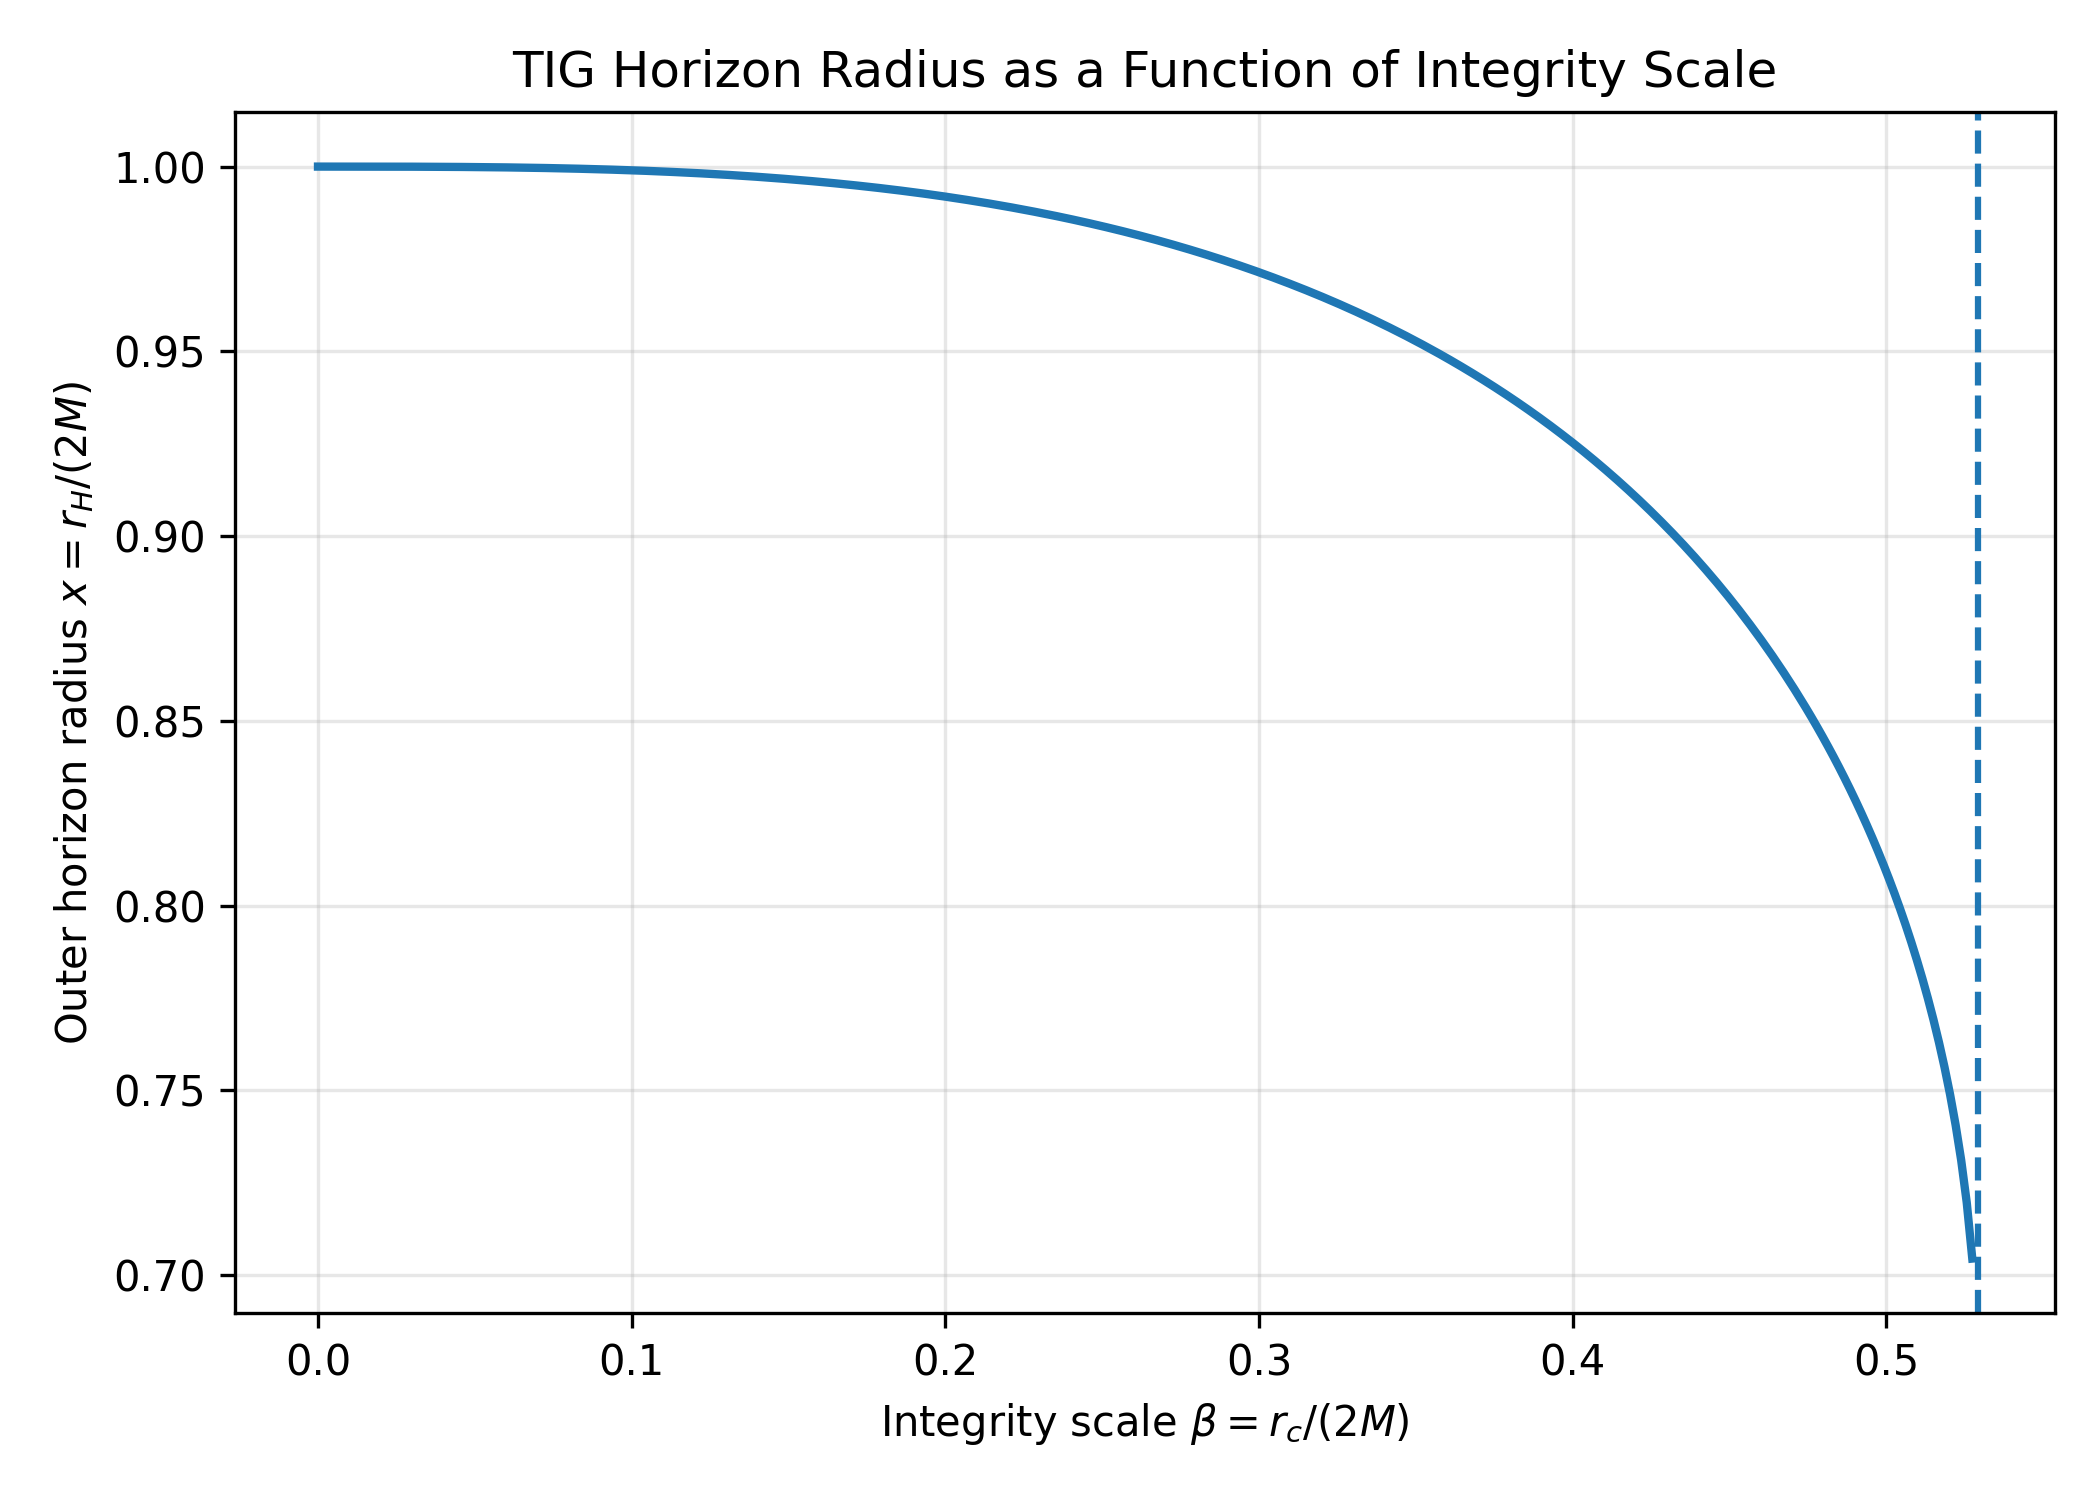
\includegraphics[width=0.75\textwidth]{tig_horizon_radius_prediction.png}
\caption{Horizon-radius behavior as a function of the control parameter $\beta$. The critical regime separates horizon-bearing from horizonless configurations.}
\label{fig:horizon}
\end{figure}

For small $\beta$, the outer horizon branch satisfies
\begin{equation}
x\simeq 1-\beta^3,
\end{equation}
and therefore
\begin{equation}
r_H\simeq 2M(1-\beta^3).
\end{equation}

\section{Photon Sphere}

The photon sphere is determined by
\begin{equation}
rF'(r)-2F(r)=0 .
\end{equation}

The corresponding shadow radius is
\begin{equation}
R_{\mathrm{sh}}
=
\frac{r_{\mathrm{ph}}}{\sqrt{F(r_{\mathrm{ph}})}} .
\end{equation}

Near the critical regime, deviations in photon-sphere structure may translate into observable shadow-radius deviations \cite{berti2015test}.

\section{Perturbative Dynamics}

Linear perturbations may be described by a Schrödinger-like master equation
\begin{equation}
\frac{d^2\Psi}{dr_*^2}
+
\left[
\omega^2-V_{\mathrm{eff}}(r)
\right]\Psi=0 ,
\end{equation}
where
\begin{equation}
\frac{dr_*}{dr}=\frac{1}{F(r)} .
\end{equation}

The effective potential inherits the critical behavior of the metric function.

\section{Quasi-Normal Modes}

In the eikonal approximation, quasi-normal-mode frequencies are controlled by the photon-sphere frequency and the Lyapunov exponent \cite{kokkotas1999,berti2009}:
\begin{equation}
\omega_n
\simeq
\left(n+\frac{1}{2}\right)\Omega_{\mathrm{ph}}
-
i\left(n+\frac{1}{2}\right)\lambda_{\mathrm{ph}} .
\end{equation}

Approaching the critical regime can shift both the real oscillation frequency and the damping rate.

\section{Echo Physics}

For horizonless configurations, the inner boundary is no longer purely absorbing. The characteristic echo delay is estimated as
\begin{equation}
\Delta t_{\mathrm{echo}}
\simeq
2\int_{r_0}^{r_{\mathrm{ph}}}\frac{dr}{F(r)} .
\end{equation}

Near the critical value,
\begin{equation}
\Delta t_{\mathrm{echo}}\rightarrow\infty
\qquad
\mathrm{as}
\qquad
\beta\rightarrow\beta_c .
\end{equation}

This corresponds to the formation of an effectively infinite optical cavity and is analogous to critical slowing down in dynamical systems.

\begin{figure}[H]
\centering
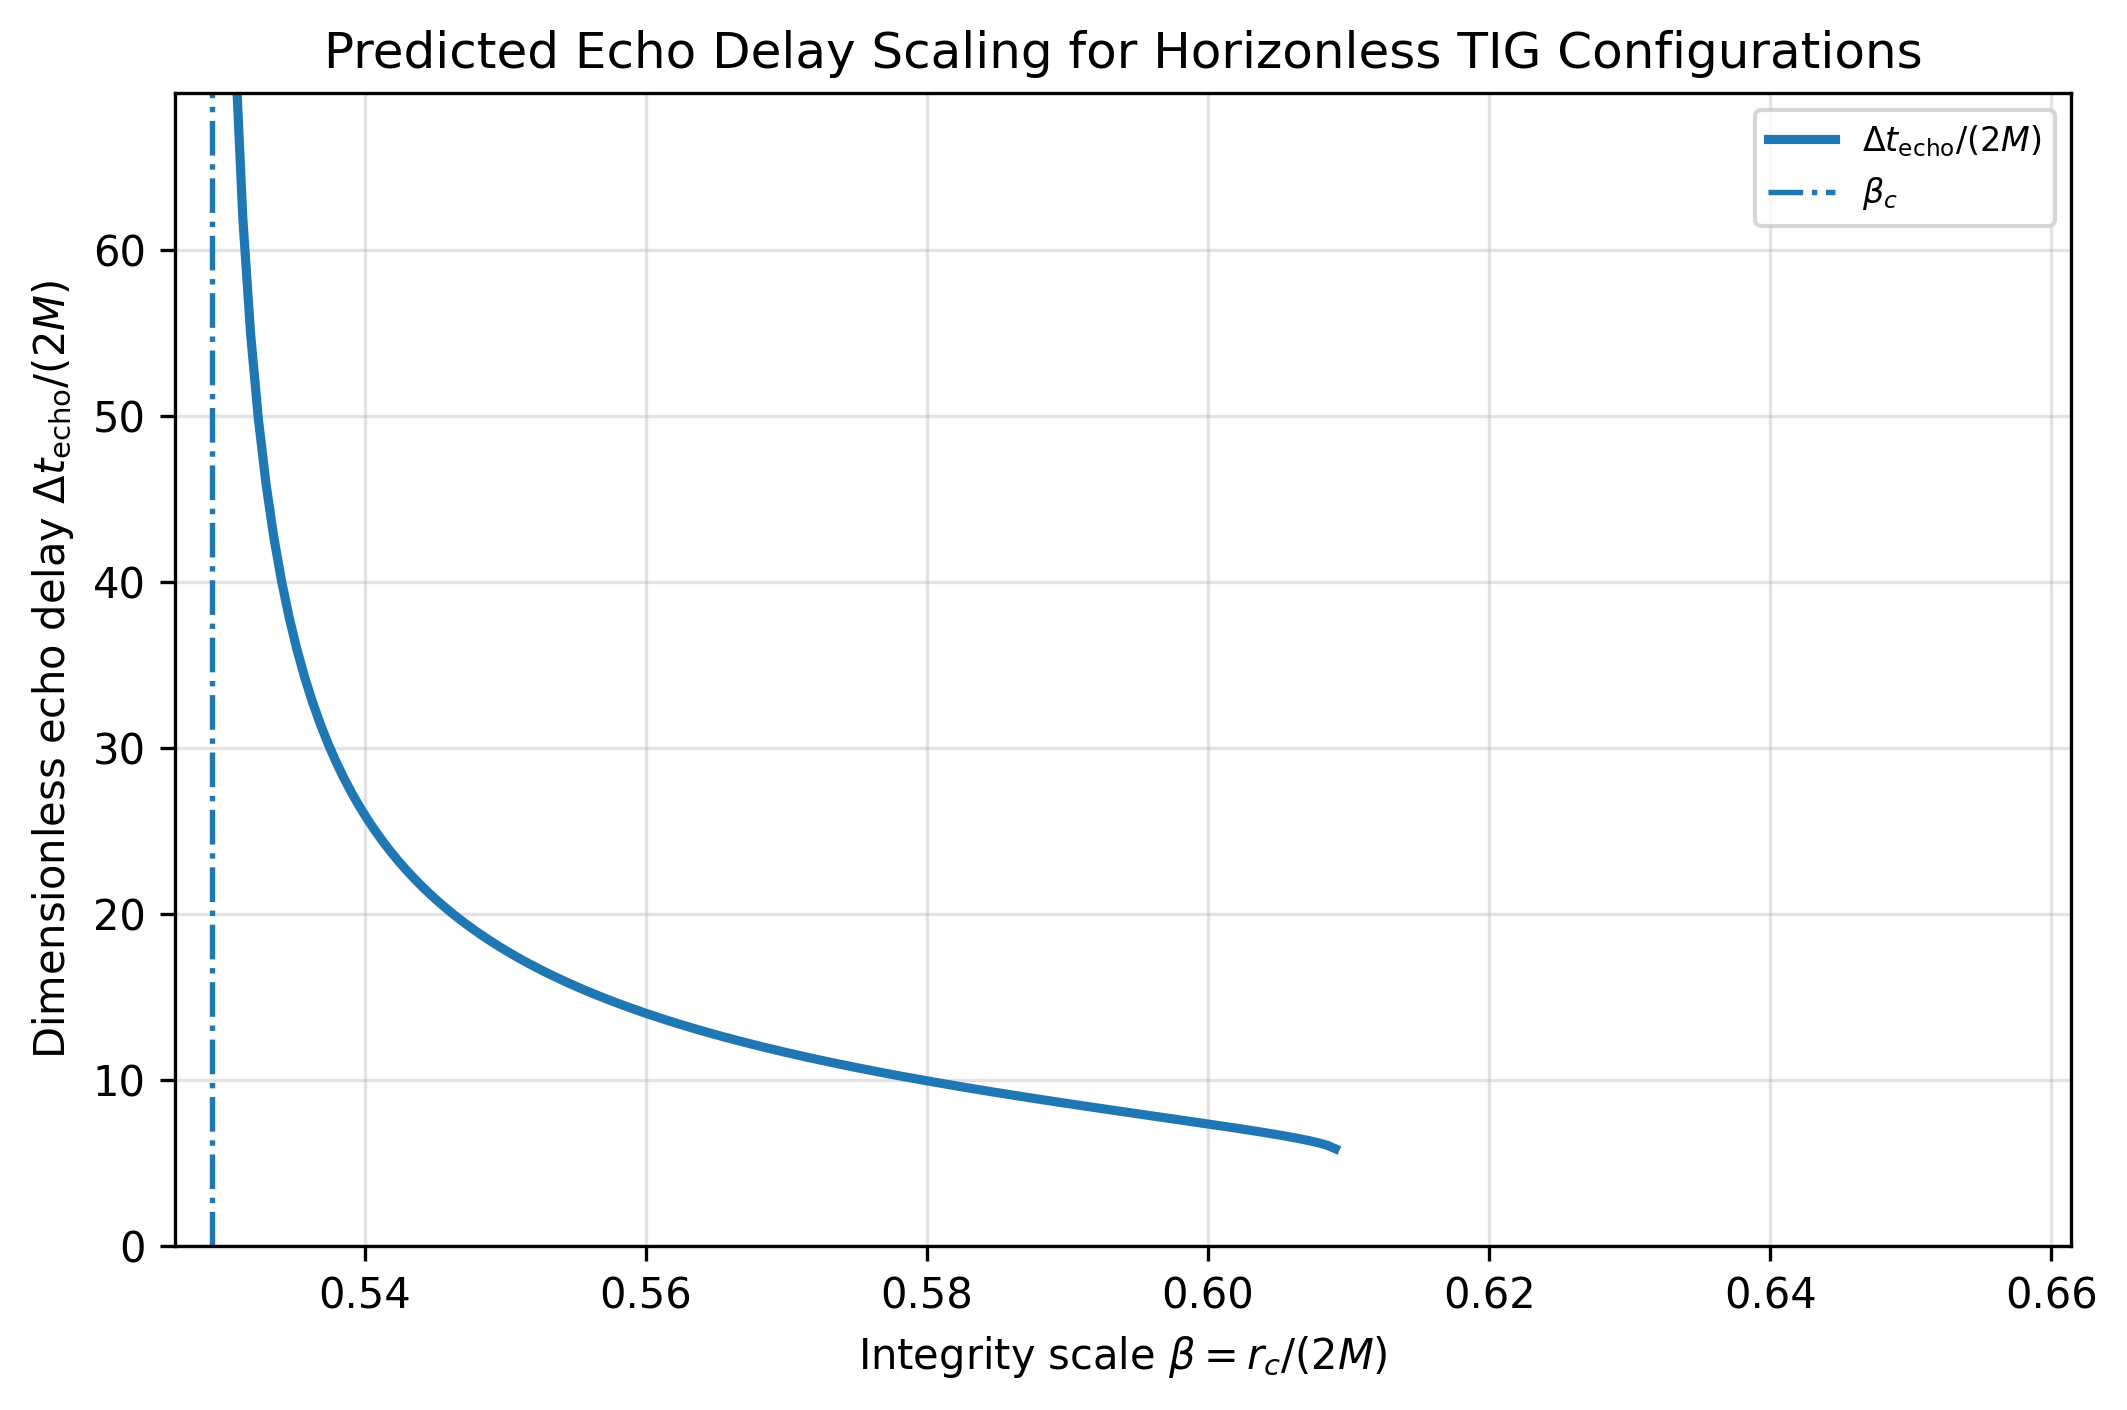
\includegraphics[width=0.75\textwidth]{tig_echo_delay_prediction.png}
\caption{Echo-delay scaling near the critical regime. The delay grows as the effective optical cavity becomes increasingly extended.}
\label{fig:echo}
\end{figure}

\section{Observational Implications}

Observable channels include:
\begin{itemize}
\item black hole shadow-radius deviations,
\item quasi-normal-mode frequency shifts,
\item possible gravitational-wave echo signatures \cite{cardoso2017echo,cardoso2017status}.
\end{itemize}

These effects provide possible probes of modified gravity in strong-field regimes \cite{berti2015test}.

\section{Stability}

For $\mu>0$, the scalar curvature mode is non-tachyonic, which supports perturbative consistency of the quadratic correction. A complete dynamical stability analysis remains future work.

\section{Relation to Regular Black Hole Models}

The effective geometry resembles regular black hole models in that the central singularity is replaced by a regular core \cite{bardeen1968,hayward2006}. However, the present construction emphasizes the analytic critical transition in horizon formation rather than only regularization of the central region.

\section{Conclusion}

We identified a structurally controlled critical transition governing horizon formation in a quadratic $f(R)$ gravity model. The transition separates horizon-bearing and horizonless configurations and leads to observable signatures in photon-sphere structure, quasi-normal-mode behavior, and echo-delay scaling.

Future work should address full numerical solutions, stability, and direct comparison with observational data.

\clearpage

\nocite{*}
\bibliographystyle{unsrt}
\bibliography{references}

\end{document}
